\section{Functies en afgeleiden}



\subsection{Functies}

Eén van de centrale concepten binnen de wiskunde, en zeker zeker ook binnen de \textit{machine learning} is de \textit{functie}. Formeel beschrijft een functie een relatie tussen twee verzamelingen $X$ en $Y$, waarbij een element uit $X$ gekoppeld wordt aan precies één element uit de verzameling $Y$. Denk bijvoorbeeld aan een functie die een getal (de \textit{input}) omzet in het kwadraat van dat getal (de \textit{output}) – de functie kun je dan opvatten als een machine die kwadraten van getallen maakt, met getallen als input. 

In deze zin is een functie iets strikter dan zoals we die kennen uit onze programmeerervaring. In de wiskundige zin van het woord heeft een functie een heel duidelijke input- en output-variabele: louter op basis van de input wordt een heel strikte output bepaald, waarbij er geen \textit{side effects} optreden en zonder dat er wordt gekeken naar een staat die buiten de functie ligt (zoals systeemgegevens of klasse-variabelen).

In de regel wordt de input aangegeven met $x$ en de output met $y$. Om aan te geven dat $y$ van $x$ afhankelijk is, schrijf je de \textit{vergelijkingsvorm} $y=formule$, bijvoorbeeld $y=2x+3$. Een andere notatievorm is de \textit{haakjesvorm}: $f(x) = 2x+3$ – de functiewaarde van $y$ is gelijk aan $2x+3$. Het grote voordeel van die tweede notatievorm is dat je de functie expliciet een naam geeft, waarmee je eraan kunt referen – je spreekt dan over functie $f$ of functie $g$. Zeker wanneer je met meerdere functies tegelijk aan het werk bent, is dat onontbeerlijk. 

Behalve het geven van een formule kun je een functie natuurlijk ook in een assenstelsel tekenen. Hierbij zetten we de $x$ op de horizontale lijn en de $y$ op de verticale lijn. Elk punt in onze formule geven we dan weer als het \textit{tupel} $(x,y)$. Door al deze punten met elkaar te verbinden, verkrijgen we de grafiek van onze functie:

\begin{figure}[h!]
    \centering
    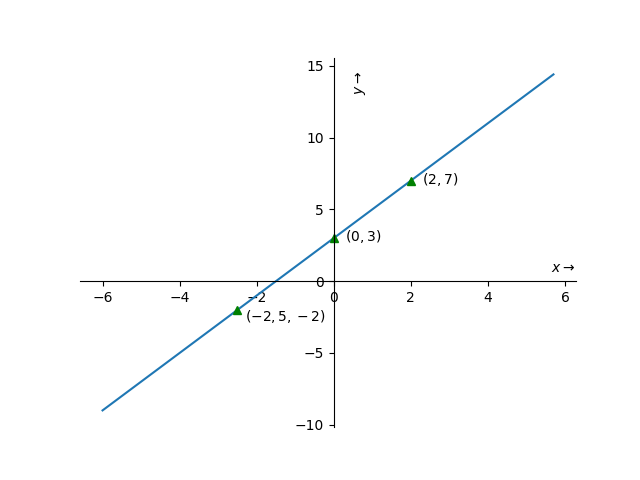
\includegraphics[width=.5\textwidth]{functie}
    \caption{Voorbeeld van een grafiek van een functie.\label{img:functie}}
\end{figure}

De verzameling van alle mogelijke waarden van de input is het \textit{domein} van de functie, dat we aangeven met $D$; de verzameling van de mogelijke waarden van de \textit{output} is het \textit{bereik} van die functie, wat wordt weergegeven met $B$. Gegeven een functie $f(x)=\sqrt{x-1}$, dan is het \textit{domein} van die functie de verzameling van alle getallen groter dan of gelijk aan 1, terwijl het \textit{bereik} van die functie gelijk is aan alle getallen groter dan of gelijk aan 0. Een dergelijke verzameling van getallen kun je omschrijven als een \textit{interval}: als $a < b$ dan vormen alle getallen tussen $a$ en $b$ het \textit{open interval} $\left(a,b\right)$. Als de getallen $a$ en $b$ ook bij het interval horen, dan spreek je van een \textit{gesloten interval}, wat je schrijft als $\left[a,b\right]$.

\begin{figure}[h]
\centering
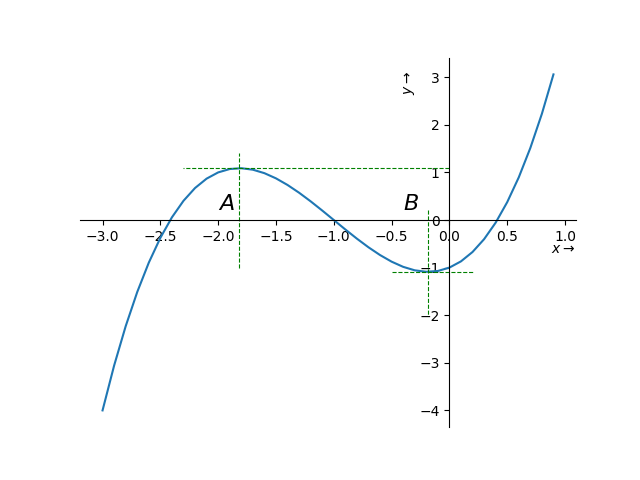
\includegraphics[width=.75\textwidth]{min_max}
\caption{Een functie met een minumum en een maximum.\label{img:min_max}}
\end{figure}

Een functie kan op een bepaald interval \textit{stijgen}, \textit{dalen}, of \textit{gelijk blijven}. Een stijging of daling kan constant zijn, toenemen of afnemen. Het punt waarop een functie van een stijging overgaat naar een daling heet een \textit{maximum}; het punt waar een functie overgaat van een daling naar een stijging heel een \textit{minimum}. Zo heeft de functie in Figuur \ref{img:min_max} een maximum in punt $(A, f(A))$ en een minumum in punt $(B, f(B))$. De functie vertoont een \textit{stijging} tussen $\left[-\infty, A \right)$ en tussen $\left( B, \infty \right]$; hij \textit{daalt} tussen $\left[A,B\right]$. Verder is zowel het \textit{domein} als het \textit{bereik} van deze functie $\left[-\infty, \infty\right]$.

\subsection{Machtfuncties en polynomen}

Een \textit{machtsfunctie} is een functie waarvan de algemene vorm $f(x)= a \cdot x^n$ is, waarbij $a$ (de \textit{vermenigvuldigingsfactor} en $n$ (de \textit{exponent}) willekeurige positieve of negatieve getallen kunnen zijn. Voor het gemak gaan we er hier van uit dat $n$ altijd een geheel positief getal is (wat voor polynomen ook wel gebruikelijk is, en anders introduceren we te veel complexiteit die voor het onderwerp \textit{machine learning} niet relevant is).

\begin{figure}[h]
    \centering
    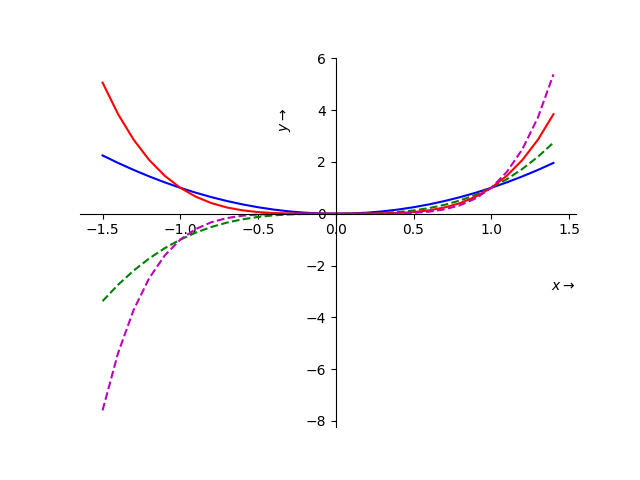
\includegraphics[width=.75\textwidth]{machtsfuncties}
    \caption{Diverse machtsfuncties bij elkaar getekend.\label{img:machtsfuncties}}
\end{figure}

In Figuur \ref{img:machtsfuncties} zijn de grafieken van $x^2$ (blauwe lijn), $x^3$ (groene stippellijn), $x^4$ (rode lijn) en $x^5$ (magenta stippellijn) getekend. Als je goed naar deze grafieken kijkt, valt een aantal zaken op. Alle vier de functies gaan door de punten $(0,0)$ en door $(1,1)$. Het bereik van de functies waarvan de exponent een \textit{even getal} is, ligt boven de y-as ($f(x) \geq 0$ voor alle $x \in D$) en deze functies zijn \textit{lijnsymmetrisch} in de y-as (dus $f(-x) = f(x)$ voor alle $x \in D$). Verder gaan deze functies allemaal door het punt $(-1, 1)$. De functies waarvan de exponent een \textit{oneven getal} is, gaan allemaal door punt $(-1,-1)$ en zijn \textit{puntsymmetrisch} in punt $(0,0)$ (dus $f(-x)=-f(x)$ voor alle $x \in D$).

Vaak zie je, zeker in het geval van \textit{machine learning}, dat een functie bestaat uit een aantal \textit{termen} met verschillende machten, zoals bijvoorbeeld de functie $f(x) = x^3+3x^2+2x$, die is weergegeven in Figuur \ref{img:polynoom}; deze functie heeft drie termen, waarvan $x^3$ de hoogste is. Zo'n soort functie noemen we een \textit{polynoom} (van het Griekse polús (veel) en nomós (deel): een functie die uit veel delen bestaat). Je ziet hier dat $f(x)=0$ voor $x=-2$, $x=-1$ en $x=0$ (de \textit{nulpunten}). Verder zitten er tussen de nulpunten een minimum en een maximum (hoewel die niet exact midden tussen de nulpunten in liggen). 

Wanneer we waarden van $x$ nemen die heel groot of heel klein zijn, heeft de hoogste term in de functie-definitie de sterkste invloed op de waarden van $f(x)$ – de functie gaat nagenoeg gelijk lopen met de functie $g(x)=x^3$. Alleen dicht bij de 0 zijn er wat verschillen waar te nemen. Deze functie wordt om die reden een polynoom van de \textit{derde graad} genoemd: de hoogste exponent van de functie-definitie bepaalt de \textit{graad} van de functie.

\begin{figure}[h]
    \centering
    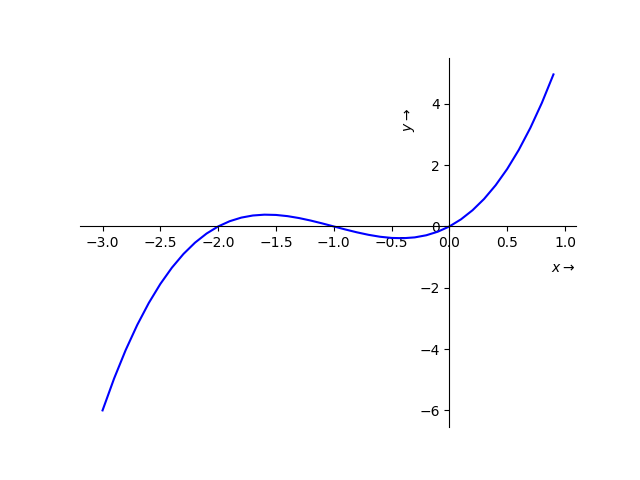
\includegraphics[width=.75\textwidth]{polynoom}
    \caption{Een polynoom van de derde graad.\label{img:polynoom}}
\end{figure}

Net als bij enkelvoudige functies kunnen de termen in een polynoom voorzien worden van een vermenigvuldigingsfactor. Zo heeft de term $x^2$ in de polynoom in Figuur \ref{img:polynoom} een vermenigvuldigingsfactor van 3 en de term $x$ een vermenigvuldigingsfactor van 2 (feitelijk is de vermenigvuldigingsfactor van de term $x^3$ gelijk aan 1, dus dat laten we weg). Het is gebruikelijk om voor het beschrijven van deze factoren dezelfde letter te gebruiken, en die te voorzien van de term waar deze bij hoort als subscript. Zo wordt de algemene beschrijving van een polynoom gegeven door $f(x) = a_nx^n + a_{n-1}x^{n-1} + a_{n-2}x^{n-2}+ \dots + a_1x^1+a_0$: dit is dan een polynoom van de n-de graad.


\subsection{Afgeleide functies}

Vaak is het van belang om te weten of een functie op een interval $\left[a,b\right]$ stijgt of daalt – de zogenaamde \textit{differentie} (het \textit{verschil} van de functiewaarden op dit interval). Om dit te bepalen, kunnen we de waarde van $f(x)$ (of $y$) voor zowel $a$ als $b$ uitrekenen en van elkaar aftrekken (waarbij $a<b$). Als $f(a) > f(b)$, dan is de differentie van $f(x)$ op $\left[a,b\right]$ \textit{negatief}: de functie vertoont een daling op het interval. Omgekeerd, als $f(a) < f(b)$, dan is de differentie van $f(x)$ op $\left[a,b\right]$ \textit{positief}: de functie vertoont een stijging. De totale differentie geven we aan met de griekse hoofdletter delta: \Delta.

\begin{figure}[h]
    \centering
    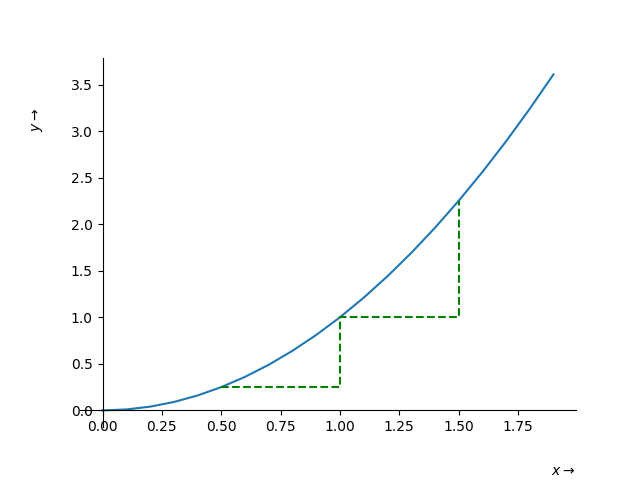
\includegraphics[width=.5\textwidth]{parabool_differentie}
    \caption{De functie $f(x) = x^2$\label{img:parabool_differentie}}
\end{figure}

In figuur \ref{img:parabool_differentie} is de functie $f(x)=x^2$ getekend voor het domein $\left[0,2\right]$. Stel nu dat we de differentie willen weten op het interval $\left[0.5, 1.0\right]$, zoals aangegeven door de linker groene stippellijn. Om dat te bepalen, berekenen we eerst $f(x)$ voor het rechter extreem van dit interval: $f(x) = x^2 = 1^2 = 1$ en vervolgens de functiewaarde van het linkerextreem van het interval: $f(x) = x^2 = (0.5)^2 = 0.25$. Vervolgens trekken we beide getallen van elkaar af om de totale differentie te verkrijgen: $1-0.25=0.75$. Op eenzelfde manier verkrijgen we de differentie op het interval $\left[1, 1.5\right]$: $\Delta = f(x_2) - f(x_1) = f(1.5)-f(1) = 2.25-1 = 1.25$, die met de rechter groene lijntjes is aangegeven.

    
Behalve het totaal is ook de \textit{gemiddelde} stijging of daling van belang – het zogenaamde \textit{differentiequotiënt} – de deling (het \textit{quotiënt}) van de verschillen (de \textit{differenties}) tussen de beide $x$-en en de beide $y$-en. Dit berekenen we door de totale stijging of daling op een interval te delen door de lengte van het interval. Het differentiequotiënt van $f(x)$ uit Figuur \ref{img:parabool_differentie} op het interval $\left[0.5,1\right]$ is dus $\frac{1-0.25}{1-0.5} = \frac{0.75}{0.5} = 1.5$. Dit cijfer correspondeert met de \textit{richtingscoëfficiënt} van de lijn die de beide extremen van het gegeven interval met elkaar verbindt – de rode stippellijn in Figuur \ref{img:parabool_ricos}. Op een vergelijkbare manier kunnen we de richtingscoëfficiënt van de lijn in het tweede interval berekenen: de magenta lijn in de figuur. 

\begin{figure}[h]
    \centering
    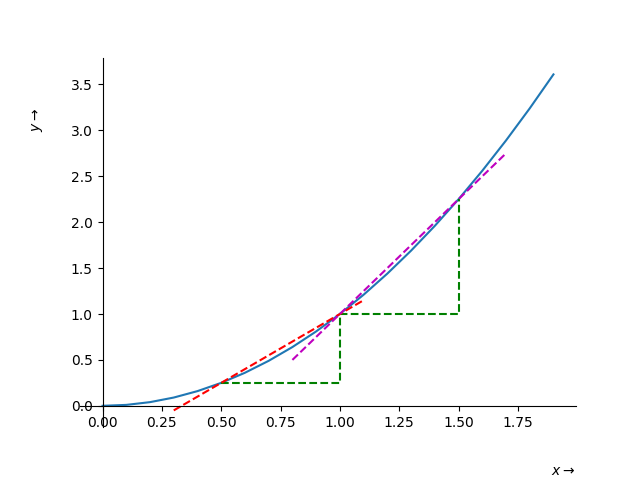
\includegraphics[width=.5\textwidth]{parabool_ricos}
    \caption{De functie $f(x) = x^2$, intervallen voorzien van raaklijnen\label{img:parabool_ricos}}
\end{figure}

Algemeen geldt dat als $a<b$, het differentiequotiënt gelijk is aan

\[
    \frac{f(b)-f(a)}{b-a}.
\]

Om de differentie van een functie op een specifiek punt $f(a)$ te bepalen, berekenen we de gemiddelde differentie van de functie op het interval $\left[a,a+h\right]$, waarbij we $h$ steeds kleiner maken (alsof we de rechter groene lijnen in Figuur \ref{img:parabool_ricos} steeds dichter bij de linkerlijnen laten komen). Stel nu dat $f(x)=x^2$, dan kunnen we differentie op punt $x$ als volgt bepalen:
\[
\begin{aligned}
    \Delta &= \frac{f(x+h)-f(x)}{(x+h) - x} & \text{waarden voor } x \text{ en } h \text{ invullen:}\\
    &= \frac{(x+h)^2 - x^2}{(x+h)-x} & \text{kwadraten uitwerken en noemer versimpelen:} \\
    &= \frac{(x^2 + 2xh + h^2)-x^2}{h} & \text {teller vereenvoudigen:} \\
    &= \frac{2xh + h^2}{h} & \text{alles delen door h:} \\
    &= 2x + h & \text{h nadert tot nul:} \\
    &= 2x
\end{aligned}
\]            

(Zoals je ziet zit er in deze afleiding een opvallende stap, namelijk wanneer we beide termen delen door $h$. Dit kan natuurlijk niet zonder meer, zeker niet omdat we $h$ laten naderen tot 0. Het voert te ver om hier toe te lichten waarom dat in dit geval toegestaan is, omdat we niet echt delen door nul, maar $h$ steeds dichter naar nul laten naderen (maar het wordt dus nooit echt helemaal nul). Zie voor meer informatie \href{https://www.wisfaq.nl/pagina.asp?nummer=1451}{deze link}.)

We zien dus dat de differentie van elk punt $x$ op de functie $f(x) = x^2$ zelf ook weer een functie van $x$ is, namelijk $2x$. 
Deze tweede functie heet de \textit{afgeleide functie} van $f(x)$ en wordt genoteerd als $f'(x)$, of als een zogenaamd \textit{differentiequotiënt}:

\[
    f'(x) = \frac{df}{dx}
\]

Het bepalen van een afgeleide functie wordt \textit{differentiëren} genoemd; de grafiek van $f'(x)$ heet de \textit{hellingsgrafiek} van $f(x)$. Differentiëren is een tak van de wiskunde die behoorlijk complex kan worden, maar voor nu volstaan de volgende algemene regels:

\begin{itemize}
    \item De hellingsgrafiek van de functie $f(x)=0$ is de lijn $f'(x)=0$: de verandering is overal 0.
    \item De hellingsgrafiek van een constante functie $f(x)=x$ is de lijn $f'(x)=1$: de verandering blijft overal hetzelfde.
    \item De hellingsgrafiek van een niet-horizontale lijn $f(x) = ax + b$ is de constante functie $f'(x)=a$: het lokale verandering van functiewaarden is overal hetzelfde. 
    \item In het algemeen geldt dat als $f(x) = x^n$, dan is $f'(x) = nx^{n-1}$. 
\end{itemize}

Wanneer we een functie $f(x)$ met domein $D$ hebben, noemen we deze functie \textit{differentieerbaar} wanneer we voor elke $x \in D$ een afgeleide waarde kunnen bepalen. Zo is de functie $f(x) = x^2$ differentieerbaar, want over het hele domein ($D = \left[-\infty, \infty\right]$) kunnen we een afgeleide waarde bepalen, namelijk $f'(x)=2x$. De functie $f(x)=|x|$ (zie Figuur \ref{img:abs}) is daarentegen niet differentieerbaar: de afgeleide functie hiervan is $f'(x)=-1 (x<0)$ en $f'(x)=1 (x>0)$, maar voor $x=0$ is de afgeleide waarde ongedefinieerd: je kunt immers oneindig veel lijnen trekken die allemaal het punt $(0,0)$ raken (in de figuur zijn twee voorbeelden getekend – de groene stippellijnen).

\begin{figure}[h]
    \centering
    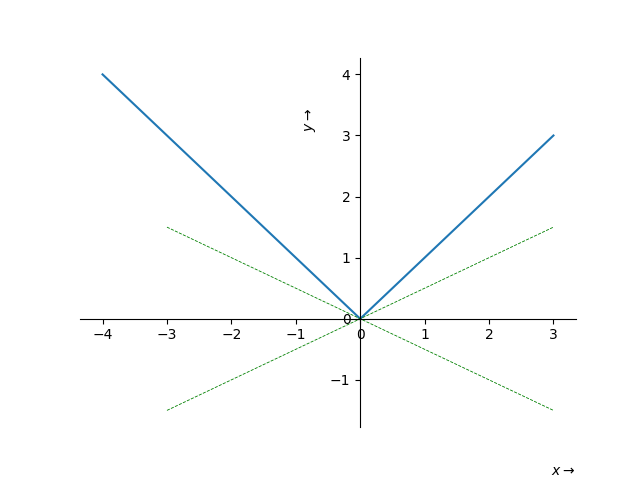
\includegraphics[width=.75\textwidth]{absoluut}
    \caption{De functie $f(x) = |x|$\label{img:abs}}
\end{figure}
